%#################################################################
\chapter{DSL para a Representação de Modelos Conceituais de Banco de Dados Relacionais}\label{propostaDSL}
%#################################################################
\addlinespace
Este capítulo apresenta a proposta central deste trabalho. 
A Seção \ref{sec:reqDSL} aponta os requisitos levantados para a construção da \ac{DSL}. 
A Seção \ref{sec:decDSL} descreve as decisões de projeto referentes aos requisitos. 
A arquitetura da implementação da proposta é detalhada na Seção \ref{sec:arqDSL}. 
A demonstração do protótipo construído ocorre na Seção \ref{sec:protDSL}.
Em seguida a avaliação preliminar conduzida com um grupo focal é apresentado na Seção \ref{sec:AvalPrelGram}, bem como os resultados obtidos.
A Seção \ref{sec:ERTEXTFinal} detalha a ferramenta ERText, produto do desenvolvimento da \ac{DSL} e, por fim, as lições do capítulo são pontuadas na Seção \ref{sec:licDSL}.

%#################################################################
\section{Requisitos da Linguagem} \label{sec:reqDSL}
%#################################################################

Esta seção lista os requisitos que foram definidos com base na literatura utilizada neste trabalho, bem como no conhecimento prévio dos pesquisadores envolvidos na condução do estudo. 
Estes requisitos são relacionados diretamente com as decisões de projeto.

\begin{itemize}

\item\textit{\textbf{RQ1. A \ac{DSL} precisa ser disponibilizada sob uma licença open source.}} 
Como o foco da proposta é no processo de ensino é fundamental que a linguagem seja de código aberto. 
A vantagem que este requisito proporciona é a posterior evolução e manutenção colaborativa com o envolvimento de outros desenvolvedores.

\item\textit{\textbf{RQ2. A \ac{DSL} deve permitir representar textualmente modelos conceituais de \acp{BD}.}} 
Como é um objetivo que a solução seja outra opção em relação às abordagens gráficas, esse requisito se justifica. 
Isso permite o foco na compreensão do domínio e no desenvolvimento da \ac{DSL}.

\item\textit{\textbf{RQ3. Os modelos conceituais devem dar suporte à definição de entidades, atributos, relações e cardinalidades.}} 
As ferramentas utilizadas para o desenvolvimento da linguagem precisam permitir que sejam implementados os conceitos de domínio que regem a estrutura de \ac{DER} tradicional.

\item\textit{\textbf{RQ4. Os modelos conceituais devem dar suporte a definição de atributos identificadores, generalização/especialização, auto-relacionamentos e relacionamentos ternários.}} 
A linguagem deve permitir que conceitos mais sofisticados dos domínios sejam definidos.

\item\textit{\textbf{RQ5. A implementação da \ac{DSL} deve realizar a transformação do modelo conceitual para o lógico.}} 
A solução deve realizar a transformação do conceitual para o lógico, exibindo o resultado gerado ao usuário.

% \item\textit{\textbf{RQ6. A implementação da \ac{DSL} deve gerar instruções \ac{SQL} equivalentes, com base no modelo conceitual ou lógico.}} 
% A solução precisa realizar a geração de instruções \ac{SQL} para diferentes \acp{SGBD}.

\end{itemize}

%#################################################################
\section{Decisões de Projeto} \label{sec:decDSL}
%#################################################################

Nesta seção são descritas as decisões de projeto para criar a \ac{DSL} textual que suporte todos os requisitos discutidos na Seção \ref{sec:reqDSL}. 
Para cada decisão de projeto são indicados os seus requisitos associados.

\begin{itemize}
    \item\textit{\textbf{DP1. A solução deve adotar um \ac{LW} open source no auxílio da implementação da \ac{DSL} textual (RQ1, RQ2).}} 
    Mediante a investigação conduzida durante este estudo foi selecionado o \ac{LW} Xtext para o desenvolvimento da proposta por ser um \textit{framework open source} focado no desenvolvimento de \acp{DSL} textuais, fornecendo toda a infraestrutura necessária. 
    Além disto, o Xtext é uma ferramenta com alto nível de maturidade, documentação detalhada e uma comunidade ativa. 
    
    \item\textit{\textbf{DP2. A \ac{DSL} deve fornecer uma representação textual que seja equivalente ao modelo \ac{ER} gráfico usualmente utilizado (RQ3, RQ4).}} 
    Para os requisitos cobertos por esta decisão de projeto foi adotada a estratégia de se realizar uma análise nas ferramentas averiguadas no mapeamento descrito no \autoref{mapeamentoLiteratura}, bem como no livro referência de \citeonline{Heuser:2009}.
    
    \item\textit{\textbf{DP3. A solução deve realizar a transformação entre os modelos (RQ5).}} 
    O Xtext usa modelos do \ac{EMF} como a representação na memória de qualquer arquivo de texto analisado. 
    Esse grafo de objetos na memória é chamado de árvore sintática abstrata, do inglês \ac{AST}. 
    Esses conceitos também são chamados de gráficos de objeto de documento, do inglês \ac{DOM}, modelo semântico ou simplesmente modelo. 
    Desta forma, existe a representação do modelo da gramática na forma de um metamodelo central no núcleo do \ac{EMF}, chamado de modelo \textit{Ecore}. 
    Tendo o \textit{Ecore} da \ac{DSL} proposta como uma representação, é possível então aplicar regras de transformação, gerando assim outros modelos.
    
    % \item\textit{\textbf{DP4. A solução deve prover a integração entre a \ac{DSL} e outras tecnologias (RQ6).}} 
    % A solução deve permitir a realização da exportação dos modelos construídos para um formato de instruções \ac{SQL}, representando assim o modelo físico. 
    % Inicialmente, essa integração será realizada para o SQL Server, o MySQL e o PostgreSQL.
\end{itemize}


%#################################################################
\section{Arquitetura} \label{sec:arqDSL}
%#################################################################

O \textit{framework} Xtext gera toda a infraestrutura para a criação de linguagens com base fundamentalmente nas gramáticas definidas. 
A \autoref{fig:arqXtext} fornece uma visão geral em um nível abstrato da arquitetura do Xtext. 
% Tendo esse contexto estabelecido, começou-se a definição da \ac{DSL}. 

\begin{figure}[!htb]
    \centering
    \caption{Arquitetura geral do Xtext.}
    % 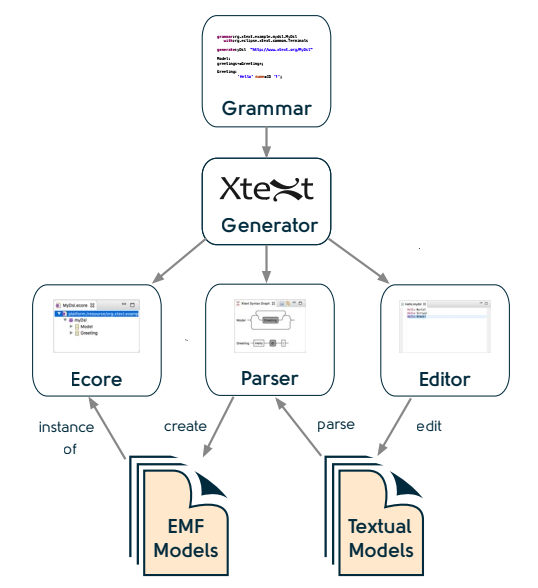
\includegraphics[width=0.6\textwidth]{img/ArquiteturaXtext.jpg}
    

\tikzset{every picture/.style={line width=0.75pt}} %set default line width to 0.75pt        

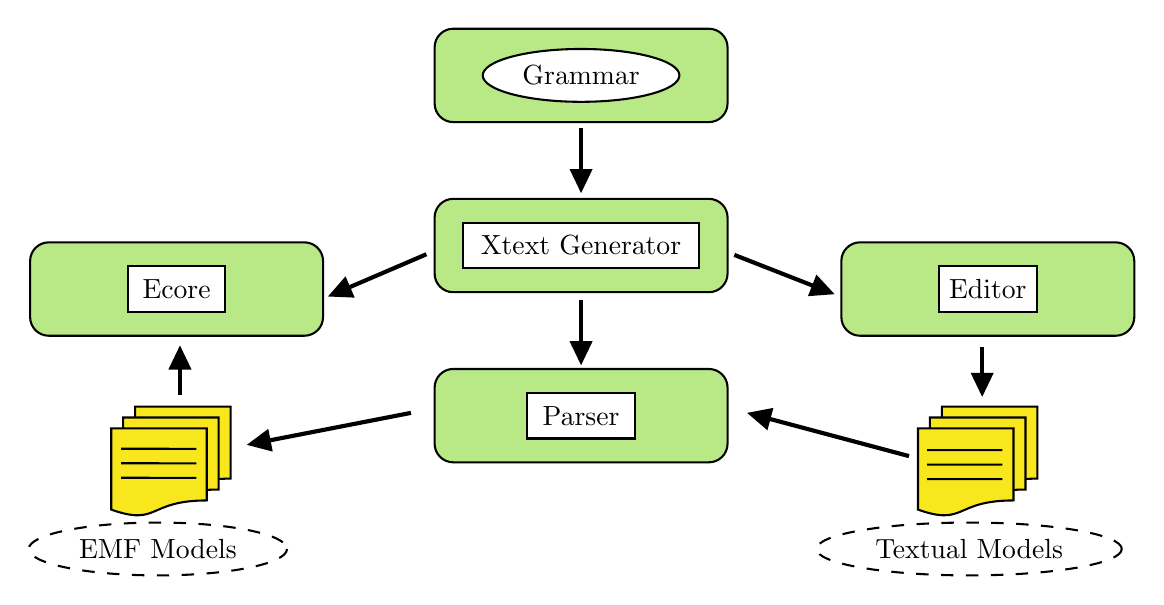
\begin{tikzpicture}[x=0.75pt,y=0.75pt,yscale=-1,xscale=1]
%uncomment if require: \path (0,440.1999969482422); %set diagram left start at 0, and has height of 440.1999969482422

%Rounded Rect [id:dp8080613887465731] 
\draw  [fill={rgb, 255:red, 184; green, 233; blue, 134 }  ,fill opacity=1 ] (268.19,31.77) .. controls (268.19,26.8) and (272.21,22.77) .. (277.18,22.77) -- (400.33,22.77) .. controls (405.3,22.77) and (409.33,26.8) .. (409.33,31.77) -- (409.33,58.76) .. controls (409.33,63.73) and (405.3,67.76) .. (400.33,67.76) -- (277.18,67.76) .. controls (272.21,67.76) and (268.19,63.73) .. (268.19,58.76) -- cycle ;

%Rounded Rect [id:dp23877247410758984] 
\draw  [fill={rgb, 255:red, 184; green, 233; blue, 134 }  ,fill opacity=1 ] (464.16,134.7) .. controls (464.16,129.73) and (468.19,125.7) .. (473.15,125.7) -- (596.3,125.7) .. controls (601.27,125.7) and (605.3,129.73) .. (605.3,134.7) -- (605.3,161.69) .. controls (605.3,166.66) and (601.27,170.69) .. (596.3,170.69) -- (473.15,170.69) .. controls (468.19,170.69) and (464.16,166.66) .. (464.16,161.69) -- cycle ;

%Rounded Rect [id:dp8660361288400333] 
\draw  [fill={rgb, 255:red, 184; green, 233; blue, 134 }  ,fill opacity=1 ] (268.19,113.73) .. controls (268.19,108.76) and (272.21,104.74) .. (277.18,104.74) -- (400.33,104.74) .. controls (405.3,104.74) and (409.33,108.76) .. (409.33,113.73) -- (409.33,140.72) .. controls (409.33,145.69) and (405.3,149.72) .. (400.33,149.72) -- (277.18,149.72) .. controls (272.21,149.72) and (268.19,145.69) .. (268.19,140.72) -- cycle ;

%Rounded Rect [id:dp8159423215616721] 
\draw  [fill={rgb, 255:red, 184; green, 233; blue, 134 }  ,fill opacity=1 ] (73.3,134.7) .. controls (73.3,129.73) and (77.33,125.7) .. (82.3,125.7) -- (205.45,125.7) .. controls (210.41,125.7) and (214.44,129.73) .. (214.44,134.7) -- (214.44,161.69) .. controls (214.44,166.66) and (210.41,170.69) .. (205.45,170.69) -- (82.3,170.69) .. controls (77.33,170.69) and (73.3,166.66) .. (73.3,161.69) -- cycle ;

%Rounded Rect [id:dp9641259565957541] 
\draw  [fill={rgb, 255:red, 184; green, 233; blue, 134 }  ,fill opacity=1 ] (268.19,195.7) .. controls (268.19,190.73) and (272.21,186.7) .. (277.18,186.7) -- (400.33,186.7) .. controls (405.3,186.7) and (409.33,190.73) .. (409.33,195.7) -- (409.33,222.69) .. controls (409.33,227.66) and (405.3,231.68) .. (400.33,231.68) -- (277.18,231.68) .. controls (272.21,231.68) and (268.19,227.66) .. (268.19,222.69) -- cycle ;

%Flowchart: Multidocument [id:dp814245162277164] 
\draw  [fill={rgb, 255:red, 248; green, 231; blue, 28 }  ,fill opacity=1 ] (123.89,204.81) -- (169.93,204.81) -- (169.93,239.53) .. controls (141.16,239.53) and (146.91,252.05) .. (123.89,243.95) -- cycle ; \draw  [fill={rgb, 255:red, 248; green, 231; blue, 28 }  ,fill opacity=1 ] (118.14,210.07) -- (164.17,210.07) -- (164.17,244.79) .. controls (135.4,244.79) and (141.16,257.31) .. (118.14,249.21) -- cycle ; \draw  [fill={rgb, 255:red, 248; green, 231; blue, 28 }  ,fill opacity=1 ] (112.39,215.33) -- (158.42,215.33) -- (158.42,250.05) .. controls (129.65,250.05) and (135.4,262.57) .. (112.39,254.47) -- cycle ;
%Straight Lines [id:da659202853659377] 
\draw    (117.13,225.14) -- (153.43,225.17) ;


%Straight Lines [id:da8271632436642871] 
\draw    (117.13,232.13) -- (153.43,232.16) ;


%Straight Lines [id:da22701123408508272] 
\draw    (117.13,239.12) -- (153.43,239.15) ;




%Flowchart: Multidocument [id:dp49717070559395604] 
\draw  [fill={rgb, 255:red, 248; green, 231; blue, 28 }  ,fill opacity=1 ] (512.58,204.81) -- (558.61,204.81) -- (558.61,239.53) .. controls (529.84,239.53) and (535.6,252.05) .. (512.58,243.95) -- cycle ; \draw  [fill={rgb, 255:red, 248; green, 231; blue, 28 }  ,fill opacity=1 ] (506.83,210.07) -- (552.86,210.07) -- (552.86,244.79) .. controls (524.09,244.79) and (529.84,257.31) .. (506.83,249.21) -- cycle ; \draw  [fill={rgb, 255:red, 248; green, 231; blue, 28 }  ,fill opacity=1 ] (501.07,215.33) -- (547.11,215.33) -- (547.11,250.05) .. controls (518.33,250.05) and (524.09,262.57) .. (501.07,254.47) -- cycle ;
%Straight Lines [id:da5642847406466045] 
\draw [fill={rgb, 255:red, 248; green, 231; blue, 28 }  ,fill opacity=1 ]   (505.45,225.77) -- (541.75,225.81) ;


%Straight Lines [id:da9779186616916171] 
\draw [fill={rgb, 255:red, 248; green, 231; blue, 28 }  ,fill opacity=1 ]   (505.45,232.76) -- (541.75,232.8) ;


%Straight Lines [id:da8217185402464098] 
\draw [fill={rgb, 255:red, 248; green, 231; blue, 28 }  ,fill opacity=1 ]   (505.45,239.75) -- (541.75,239.78) ;




%Straight Lines [id:da4555835119587406] 
\draw [line width=1.5]    (338.76,70.52) -- (338.76,98.97) ;
\draw [shift={(338.76,101.97)}, rotate = 270] [fill={rgb, 255:red, 0; green, 0; blue, 0 }  ][line width=1.5]  [draw opacity=0] (11.61,-5.58) -- (0,0) -- (11.61,5.58) -- cycle    ;

%Straight Lines [id:da2586670416419199] 
\draw [line width=1.5]    (338.76,153.44) -- (338.76,181.89) ;
\draw [shift={(338.76,184.89)}, rotate = 270] [fill={rgb, 255:red, 0; green, 0; blue, 0 }  ][line width=1.5]  [draw opacity=0] (11.61,-5.58) -- (0,0) -- (11.61,5.58) -- cycle    ;

%Straight Lines [id:da2552674310073062] 
\draw [line width=1.5]    (264.22,131.44) -- (219.57,150.59) ;
\draw [shift={(216.81,151.77)}, rotate = 336.78999999999996] [fill={rgb, 255:red, 0; green, 0; blue, 0 }  ][line width=1.5]  [draw opacity=0] (11.61,-5.58) -- (0,0) -- (11.61,5.58) -- cycle    ;

%Straight Lines [id:da29550662771480396] 
\draw [line width=1.5]    (458.11,149.58) -- (412.6,131.75) ;

\draw [shift={(460.9,150.67)}, rotate = 201.39] [fill={rgb, 255:red, 0; green, 0; blue, 0 }  ][line width=1.5]  [draw opacity=0] (11.61,-5.58) -- (0,0) -- (11.61,5.58) -- cycle    ;
%Straight Lines [id:da3813677861719633] 
\draw [line width=1.5]    (532.01,176.31) -- (532.01,197.14) ;
\draw [shift={(532.01,200.14)}, rotate = 270] [fill={rgb, 255:red, 0; green, 0; blue, 0 }  ][line width=1.5]  [draw opacity=0] (11.61,-5.58) -- (0,0) -- (11.61,5.58) -- cycle    ;

%Straight Lines [id:da3940907258410822] 
\draw [line width=1.5]    (145.5,178.36) -- (145.5,199.18) ;

\draw [shift={(145.5,175.36)}, rotate = 90] [fill={rgb, 255:red, 0; green, 0; blue, 0 }  ][line width=1.5]  [draw opacity=0] (11.61,-5.58) -- (0,0) -- (11.61,5.58) -- cycle    ;
%Straight Lines [id:da3280771928101003] 
\draw [line width=1.5]    (256.79,207.86) -- (180.67,222.68) ;
\draw [shift={(177.73,223.25)}, rotate = 348.98] [fill={rgb, 255:red, 0; green, 0; blue, 0 }  ][line width=1.5]  [draw opacity=0] (11.61,-5.58) -- (0,0) -- (11.61,5.58) -- cycle    ;

%Straight Lines [id:da9478402467031726] 
\draw [line width=1.5]    (496.73,228.68) -- (421.65,208.63) ;
\draw [shift={(418.76,207.86)}, rotate = 374.95] [fill={rgb, 255:red, 0; green, 0; blue, 0 }  ][line width=1.5]  [draw opacity=0] (11.61,-5.58) -- (0,0) -- (11.61,5.58) -- cycle    ;


% Text Node
\draw  [fill={rgb, 255:red, 255; green, 255; blue, 255 }  ,fill opacity=1 ]  (511.23,137.2) -- (558.23,137.2) -- (558.23,159.2) -- (511.23,159.2) -- cycle  ;
\draw (534.73,148.2) node  [align=left] {Editor};
% Text Node
\draw  [fill={rgb, 255:red, 255; green, 255; blue, 255 }  ,fill opacity=1 ]  (120.37,137.2) -- (167.37,137.2) -- (167.37,159.2) -- (120.37,159.2) -- cycle  ;
\draw (143.87,148.2) node  [align=left] {Ecore};
% Text Node
\draw  [fill={rgb, 255:red, 255; green, 255; blue, 255 }  ,fill opacity=1 ]  (312.76,198.19) -- (364.76,198.19) -- (364.76,220.19) -- (312.76,220.19) -- cycle  ;
\draw (338.76,209.19) node  [align=left] {Parser};
% Text Node
\draw  [dash pattern={on 4.5pt off 4.5pt}]  (134.86, 273.43) circle [x radius= 62.23, y radius= 12.73]   ;
\draw (134.86,273.43) node  [align=left] {EMF Models};
% Text Node
\draw  [dash pattern={on 4.5pt off 4.5pt}]  (525.72, 273.43) circle [x radius= 73.54, y radius= 12.73]   ;
\draw (525.72,273.43) node  [align=left] {Textual Models};
% Text Node
\draw  [fill={rgb, 255:red, 255; green, 255; blue, 255 }  ,fill opacity=1 ]  (338.76, 45.26) circle [x radius= 47.38, y radius= 12.73]   ;
\draw (338.76,45.26) node  [align=left] {Grammar};
% Text Node
\draw  [fill={rgb, 255:red, 255; green, 255; blue, 255 }  ,fill opacity=1 ]  (281.76,116.23) -- (395.76,116.23) -- (395.76,138.23) -- (281.76,138.23) -- cycle  ;
\draw (338.76,127.23) node  [align=left] {Xtext Generator};


\end{tikzpicture}

    \label{fig:arqXtext}
    \fonte{Adaptado de \citeonline{XtextSirius:2017}.}
\end{figure}

Foram implementadas duas versões da gramática no protótipo da \ac{DSL}. 
A seguir as arquiteturas dessas implementações são descritas e pontua-se as diferenças entre elas. 
Essa abordagem foi definida tendo em vista que será realizada uma avaliação preliminar junto a um grupo focal. 
A partir dos resultados dessa avaliação, objetiva-se gerar uma versão final da gramática e, consequentemente, da arquitetura.

\begin{figure}[!htb]
    \centering
    \caption{Representação do modelo \textit{Ecore} da 1\degree~versão da DSL.}
    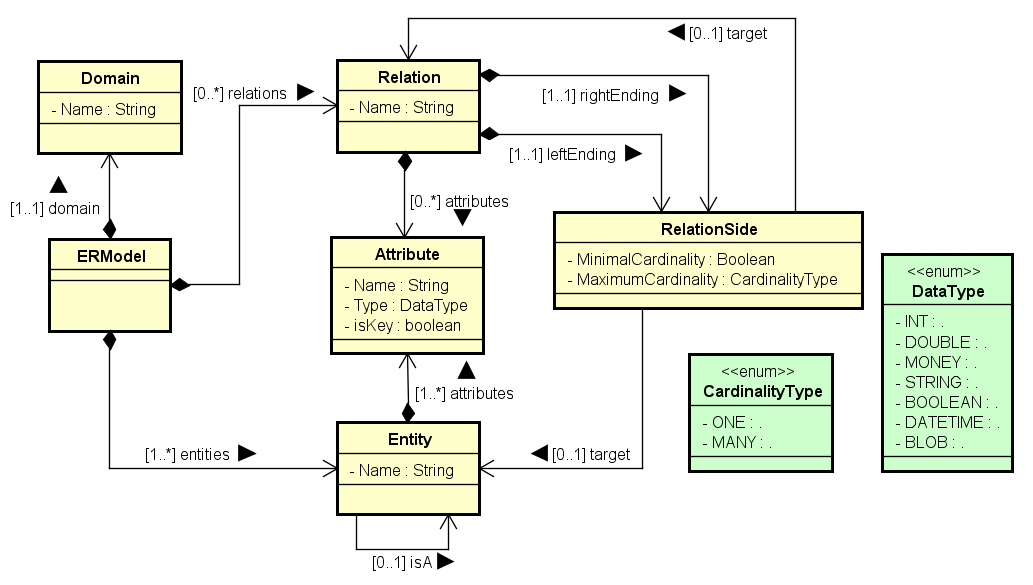
\includegraphics[width=\textwidth]{img/erDslClassDiagram.png}
    \fonte{O autor.}
    \label{fig:ERDSL}
\end{figure}

A \autoref{fig:ERDSL} mostra um diagrama de classes para representar o modelo \textit{Ecore} da primeira versão criada para esta proposta. 
O elemento central do modelo é a classe \texttt{ERModel}, a qual corresponde por uma composição com outros elementos. 
O \texttt{ERModel} deve possuir um \texttt{Domain} associado, simbolizando o nome da base de dados modelada. 

Um \texttt{ERModel} também deve conter um ou mais elementos \texttt{Entity}. 
Um elemento \texttt{Entity} pode se relacionar com outro elemento \texttt{Entity}, cobrindo assim o conceito de generalização/especialização. 
Um \texttt{Entity} é também uma composição de uma ou mais classes \texttt{Attribute}. 
Definiu-se os tipos de dados em uma lista enumerada no elemento \texttt{DataType}.

Em seguida, um \texttt{ERModel} pode ser composto de uma ou mais relações, retratado como a classe \texttt{Relation}. 
Uma \texttt{Relation} por sua vez é formada por duas classes \texttt{RelationSide}, os quais são as cardinalidades da esquerda e da direita em uma relação. 
Estas duas relações possuem uma referência chamada \texttt{Target}, que pode ser uma \texttt{Entity} ou uma \texttt{Relation}. 
A inclusão da possibilidade de se referenciar uma \texttt{Relation} se faz necessário para cobrir a modelagem dos relacionamentos ternários.

Finalmente, tem-se o conceito das cardinalidades. 
Nele as cardinalidades possíveis, mantidas em atributos da \texttt{RelationSide}, são os tipos enumerados em \texttt{CardinalityType}, sendo \texttt{One} para um e \texttt{Many} para muitos. 
Por meio das regras da gramática garante-se que a cardinalidade mínima é implícita, tendo a palavra reservada \textit{zero} para simbolizar quando uma cardinalidade mínima pode ser nula. 
Isto significa que, em uma modelagem onde uma cardinalidade mínima \textit{zero} é omitida, assume-se que ela automaticamente é igual a um.

% \begin{figure} [!htb]
%     \centering
%     \caption{Representação do modelo ECORE da segunda versão da DSL.}
%     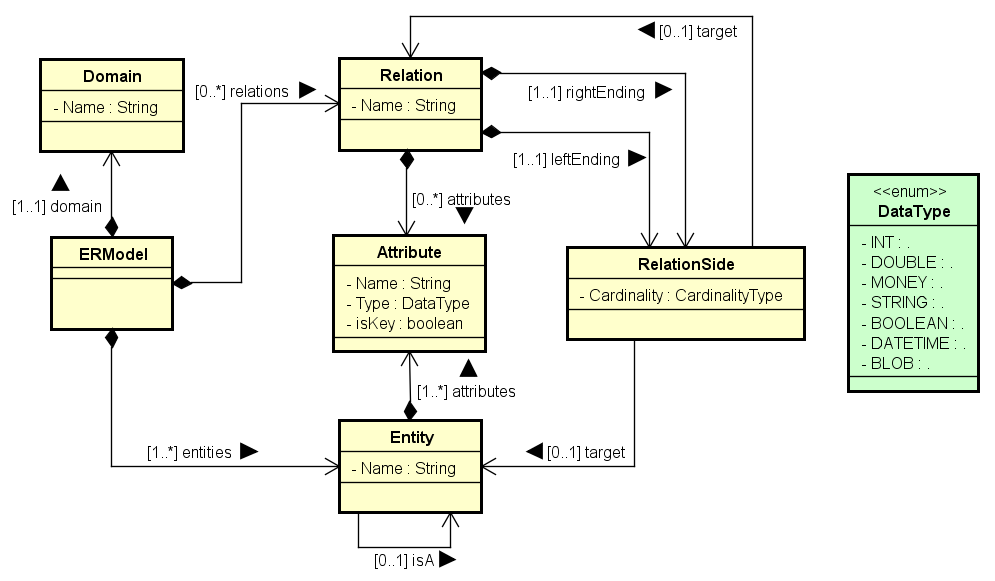
\includegraphics[width=0.8\textwidth]{img/erDsl2ClassDiagram.png}
%     \fonte{O autor.}
%     \label{fig:ERDSL2}
% \end{figure}

Estruturalmente, o modelo \textit{Ecore} da segunda versão \ac{DSL} não muda significativamente. 
%, como pode-se observar na Figura \ref{fig:ERDSL2}. 
A única diferença com maior impacto é a opção pela definição da cardinalidade utilizando-se as quatro combinações possíveis como termos reservados, armazenados diretamente no atributo \texttt{Cardinality} de \texttt{RelationSide}.

%#################################################################
\section{Protótipo} \label{sec:protDSL}
%#################################################################
\definecolor{javared}{rgb}{0.6,0,0} % for strings
\definecolor{javagreen}{rgb}{0.25,0.5,0.35} % comments
\definecolor{javapurple}{rgb}{0.5,0,0.35} % keywords
\definecolor{javadocblue}{rgb}{0.25,0.35,0.75} % javadoc
\definecolor{verde}{rgb}{0.25,0.5,0.35}
\definecolor{jpurple}{rgb}{0.5,0,0.35}
\definecolor{darkgreen}{rgb}{0.0, 0.2, 0.13}


\lstdefinelanguage{Xtext}{
  sensitive = true,
  keywords={},
  keywords=[2]{ERModel, Domain, Attribute, Entity, Relation, RelationSide, DataType, CardinalityType},
  keywords=[3]{grammar, with, generate, Terminals, enum},
  otherkeywords={*, ?, +, *=, ?=, +=, |},
  keywordstyle=\color{black}\bfseries,
  keywordstyle=[2]\color{javadocblue}\bfseries,
  keywordstyle=[3]\color{javapurple}\bfseries,% for example
%   backgroundcolor=\color{cyan!10},
%   numbers=left,
%   stepnumber=1,
  numbersep=8pt,
  showstringspaces=false,
  breaklines=true,
  frame=top,
  comment=[l]{//},
  morecomment=[s]{/*}{*/},
  commentstyle=\color{black}\ttfamily,
  stringstyle=\color{javared}\ttfamily,
  morestring=[b]',
  morestring=[b]"
  }
  
  \lstdefinelanguage{ERDSL}{
  sensitive = true,
  keywords={},
  keywords=[2]{Domain, Entities, Relationships, isIdentifier, isRelatedWith, isA, zero, one, many},
  keywords=[3]{int, money, string, datetime, file},
  otherkeywords={*, ?, +, *=, ?=, +=, |},
  keywordstyle=\color{black}\bfseries,
  keywordstyle=[2]\color{javapurple}\bfseries,
  keywordstyle=[3]\color{javadocblue}\bfseries,% for example
%   backgroundcolor=\color{cyan!10},
%   numbers=left,
%   stepnumber=1,
  captionpos=t,
  numbersep=8pt,
  showstringspaces=false,
  breaklines=true,
  frame=top,
  comment=[l]{//},
  morecomment=[s]{/*}{*/},
  commentstyle=\color{black}\ttfamily,
  stringstyle=\color{javared}\ttfamily,
  morestring=[b]',
  morestring=[b]"
  }
  
  \lstdefinelanguage{BNF}{
  sensitive = true,
  keywords={},
  keywords=[2]{},
  otherkeywords={::= , |, <, >},
  keywordstyle=\color{javapurple}\bfseries,
  keywordstyle=[2]\color{javapurple}\bfseries,
  keywordstyle=[3]\color{javadocblue}\bfseries,% for example
%   backgroundcolor=\color{cyan!10},
%   numbers=left,
%   stepnumber=1,
  captionpos=t,
  numbersep=8pt,
  showstringspaces=false,
  breaklines=true,
  frame=top,
  comment=[l]{//},
  morecomment=[s]{/*}{*/},
  commentstyle=\color{darkgreen}\ttfamily,
  stringstyle=\color{javared}\ttfamily,
  morestring=[b]',
  morestring=[b]"
  }
  
  
  
  

Na fase atual do trabalho a linguagem a nível conceitual não se encontra totalmente finalizada. 
Existem tópicos relativos a validação de escopo, como no caso do tratamento de referências cruzadas indesejadas e outras restrições inerentes ao modelo \ac{ER} que devem ser analisadas e então implementadas. 
A definição da \ac{DSL} criada é exibida na \autoref{fig:DSLvs1}.

\lstset{basicstyle=\scriptsiz}
\begin{figure}
    \centering
    \caption{Implementação da 1\degree versão da DSL.}
    \label{fig:DSLvs1}
    \begin{scriptsize}
    \begin{lstlisting}[language = Xtext , frame = trbl]
grammar org.xtext.unipampa.lesse.erdsl with org.eclipse.xtext.common.Terminals

generate erdsl "http://www.xtext.org/unipampa/lesse/erdsl/"

ERModel:
	domain=Domain ";"
	("Entities{") entities+=Entity+ ("};")
	("Relationships{") relations+=Relation* ("};");

Domain:
	"Domain" name=ID;

Entity:
	name=ID ("isA" isA+=[Entity])* 
	("{" attributes+=Attribute ("," attributes+=Attribute)* "}")?;

Attribute:
  name=ID ":" type=DataType (isKey?="isIdentifier")?;

Relation:
	(name=ID)? 
	("[" leftEnding=RelationSide 
	"isRelatedWith" 
	rightEnding=RelationSide "]")
	("{" attributes+=Attribute 
	("," attributes+=Attribute)* "}")*;
	
RelationSide:
	((minimalCardinality?="zero")?)	maximumCardinality=CardinalityType	
	target=[Entity] | target=[Relation];

enum DataType:
	INT="int" | DOUBLE="double" | MONEY="money" | STRING="string" | 
	BOOLEAN="boolean" | DATETIME="datetime" | BLOB="file";

enum CardinalityType:
	One="one" | Many="many";
    \end{lstlisting}
    \end{scriptsize}    
    \fonte{O autor.}
\end{figure}


O comando \texttt{grammar} especifica o nome da \ac{DSL}, enquanto a instrução \texttt{with} declara uma herança de outra linguagem. 
No caso da gramática proposta, será utilizada uma gramática padrão do Xtext, chamada \texttt{Terminals}, que fornece algumas regras predefinidas como, por exemplo, a regra \texttt{ID} para identificadores ou \texttt{INT} para inteiros. 
O comando \texttt{generate} é a instrução que produz a \ac{AST} da linguagem.

A primeira regra, chamada de regra de entrada, define como é a estrutura geral da linguagem. 
Palavras e símbolos entre aspas duplas ou simples indicam as palavras reservadas. 
Por exemplo, o objeto \texttt{Entities} é obrigatoriamente precedido de "\texttt{Entities\{}". 
Este objeto representa uma espécie de \textit{container}, sendo isto indicado por meio do operador de atribuição \texttt{+=}. 
Ele é um objeto que pode conter outros objetos, no caso um ou mais \texttt{Entity} (entidades). 
É estabelecido que cada arquivo da \ac{DSL} deve também ser composto de um \texttt{Domain} (domínio) e zero ou mais \texttt{Relation} (relações). 

Para melhor entendimento, deve-se deixar claro que a multiplicidade é indicada por \texttt{*} (zero ou muitos), \texttt{+} (um ou muitos) ou \texttt{?} (zero ou um). 
Ao não se colocar nenhum desses operadores, implicitamente espera-se então apenas uma ocorrência. 
Em relação às atribuições, quando apenas um \texttt{=} for especificado significa que o objeto da esquerda espera apenas um registro. 
Logo, para \texttt{+=} espera-se então zero, uma ou mais ocorrências. 

O objeto \texttt{Domain} é precedido de uma palavra reservada com o mesmo nome, seguido de um identificador. 
A entidade é definida pela palavra \texttt{Entity} e um nome identificador específico para este objeto. 
A definição de uma herança é opcional por meio da palavra reservada \texttt{isA}. 
Após a definição do nome, abre-se um corpo de chaves em que são especificados os atributos da entidade. 
Uma entidade deve conter ao menos um atributo, mas ele não precisa ser identificador por conta da possível existência de entidades fracas. 

As regras compostas só são realizadas devido à possibilidade de se agrupar expressões com o uso de parênteses, além da possibilidade de se utilizar outras regras por meio de referências cruzadas. 
Os colchetes entre a regra \texttt{Entity} servem para indicar que se almeja usar apenas o atributo \texttt{name} que identifica o objeto. 
% Se esse detalhe não for especificado então o compilador da linguagem interpretaria que é necessário aplicar toda a regra \texttt{Entity} novamente, ou seja, se iniciaria a definição de outra entidade entrando assim em um \textit{loop}. 
Os atributos das entidades são definidos por um nome, herdando a regra \texttt{ID} de \texttt{Terminals}, e atributos \texttt{isIdentifier} opcionais para simbolizar chaves primárias. 

A relação é definida, já dentro do corpo do bloco \texttt{Relationships}, com uma declaração opcional de sua identificação. 
Em seguida, são abertos colchetes e deve-se especificar dois elementos \texttt{RelationSide} como referência aos atributos \texttt{leftEnding} e \texttt{rightEnding}. 
Estes atributos representam os lados de uma relação. 
Estes objetos devem ser separados pela expressão \texttt{isRelatedWith}. 
Os lados da relação são definidos na regra \textit{RelationSide}, composta de dois atributos. 
O atributo \texttt{minimalCardinality} é opcional, indicado pelo operador \texttt{?}, e aceita apenas a palavra reservada \texttt{zero}. 
O atributo \texttt{maximumCardinality} aceita um objeto \texttt{CardinalityType}.

Os tipos de atributo estão contidos em uma lista enumerada chamada \texttt{DataType}, na esquerda fica a representação no modelo \textit{Ecore}. 
Na direita está a palavra reservada que é usada na linguagem. 
O símbolo condicional \texttt{|} significa o operador lógico \textit{OR} (ou) e serve para separar cada definição \texttt{<chave> = <valor>} como uma opção dentro da lista. 
Das três cardinalidades possíveis, duas estão definidas em outra lista enumerada chamada \texttt{CardinalityType}. 
Na \autoref{fig:DSLvs2} exibe a principal mudança entre as versões da \ac{DSL} proposta, a qual diz respeito a cardinalidade explícita. 
% A \autoref{fig:ERDSLSyntax} apresenta uma representação gráfica da sintaxe da primeira versão da gramática.

\lstset{basicstyle=\scriptsize}
\begin{figure}[!htb]
    \centering
    \caption{Fragmento de implementação da 2\degree versão da DSL.}
    \label{fig:DSLvs2}
    \begin{footnotesize}
\begin{lstlisting}[language = Xtext , frame = trbl]
Relation:
	(name=ID)? ("[" leftEnding=RelationSide "relates" 
	rightEnding=RelationSide "]") ("{"attributes+=Attribute 
	("," attributes+=Attribute)* "}")*;

RelationSide:
	Cardinality=("(0,1)" | "(1,1)" | "(0,N)" | "(1,N)")
	target=[Entity] | target=[Relation];
    \end{lstlisting}
    \end{footnotesize} 
    \fonte{O autor}
\end{figure}

% \begin{figure}[!htb]
%     \centering
%     \caption{Representação da sintaxe da 1\degree versão da \ac{DSL}.}
%     \label{fig:ERDSLSyntax}
%     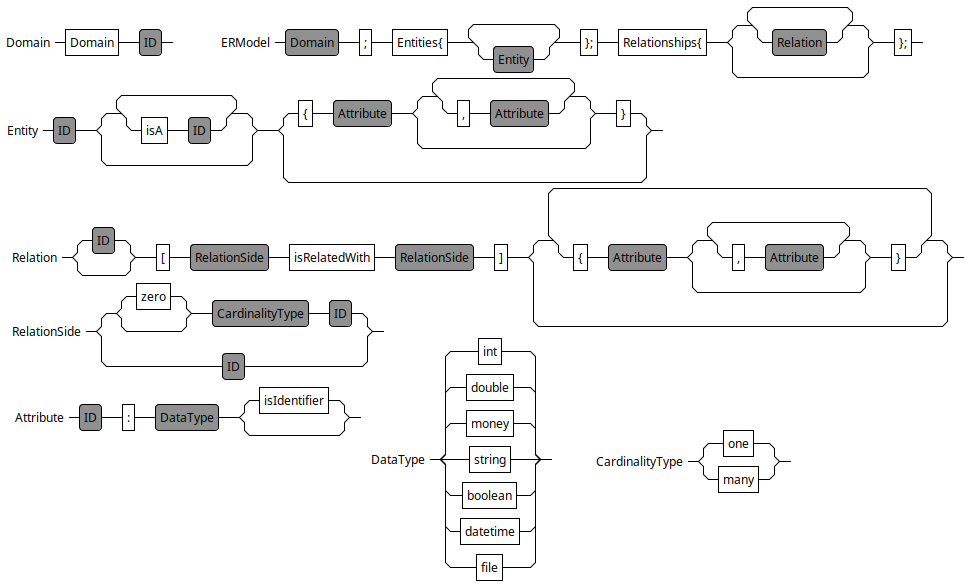
\includegraphics[width=0.9\textwidth]{img/ERDSLSyntaxGraph.png}
%     \fonte{O autor.}
% \end{figure}

% \begin{figure} [!htb]
%     \centering
%     \caption{Representação da sintaxe da 2\degree versão da \ac{DSL}.}
%     \label{fig:ERDSL2Syntax}
%     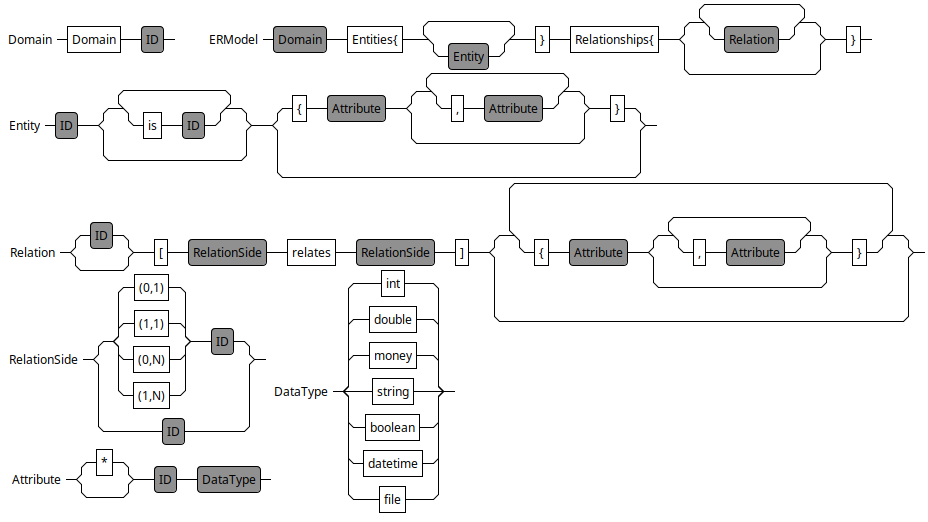
\includegraphics[width=\textwidth]{img/ERDSL2SyntaxGraph.png}
%     \fonte{O autor.}
% \end{figure}

Na \autoref{fig:DSLvs1Uso} mostra-se um exemplo de uso com um pequeno modelo que aborda uma universidade como domínio. 
Neste protótipo pode-se observar a modelagem de generalização/especialização, auto-relacionamento e relacionamento ternário.

% Para essa transformação existem regras que podem ser aplicadas, sendo que em alguns casos existem inclusive mais de uma opção. 
% Nestes casos estão sendo analisadas a melhores estratégias possíveis, uma vez que durante o processo de transformação será necessário se assumir algumas premissas.
\lstset{basicstyle=\scriptsize}
\begin{figure}[!htb]
\centering
\caption{Exemplo de uso da 1\degree versão da DSL no RCP do Eclipse.}
\label{fig:DSLvs1Uso}
\begin{scriptsize}
\begin{lstlisting}[language = ERDSL, frame = trbl]
Domain University;

Entities{
	Person{ 
		PID: int isIdentifier, 
		Name: string
	}
	Teacher isA Person{ 
		Phone: int,
		Salary:money
	}
	Student isA Person{ 
		Course: string
	} 	
	OutSrcEmployee isA Person{
	    Company: string
	}
	Class{
		ClassID: int isIdentifier,
		Course: string,
		Semester: string
	}
	ClassRoom {
		ClassRoomID: int isIdentifier,
		Capacity: int
	}
};

Relationships{	 
	[many Student isRelatedWith many Class]
	TeacherClass [many Teacher isRelatedWith many Class]
	ClassSchedule [many TeacherClass isRelatedWith many ClassRoom]
	        {CSID: int isIdentifier, DayOfWeek: datetime, Discipline: string}
	Supervisor [one OutSrcEmployee isRelatedWith many OutSrcEmployee]
};
\end{lstlisting}
\end{scriptsize}
    \fonte{O autor.}
\end{figure}
É importante destacar que neste exemplo são modeladas seis entidades e quatro relacionamentos. 
Não obstante, no processo de transformação para o modelo lógico espera-se que seja gerado um esquema textual com mais três entidades, inferindo-se isso por meio de, por exemplo, relacionamentos \textit{muitos para muitos}. 
Isso ocorreria, nesta amostra, no relacionamento sem identificação, atribuindo automaticamente a nova entidade o nome resultante da concatenação das duas entidades que se relacionam no conceitual. 
Também seriam criadas novas entidades a partir da derivação dos relacionamentos nomeados \texttt{TeacherClass} e \texttt{ClassShedule}, sendo que o último carateriza um relacionamento ternário.
Por fim, o auto-relacionamento \texttt{Supervisor} de \texttt{OutSrcEmployee} implicaria na adição de um novo atributo na entidade no novo modelo.

Com base nos modelos \textit{Ecore} gerados em tempo real, começou-se a implementar a transformação preliminar do modelo conceitual para o lógico. 
A implementação desta transformação foi realizada utilizando-se a Xtend, uma \ac{GPL} baseada em Java.

% \begin{figure} [!htb]
%     \centering
%     \caption{Fragmento do modelo \textit{Ecore} gerado em tempo de execução.}
%     \label{fig:EcoreRealTime}
%     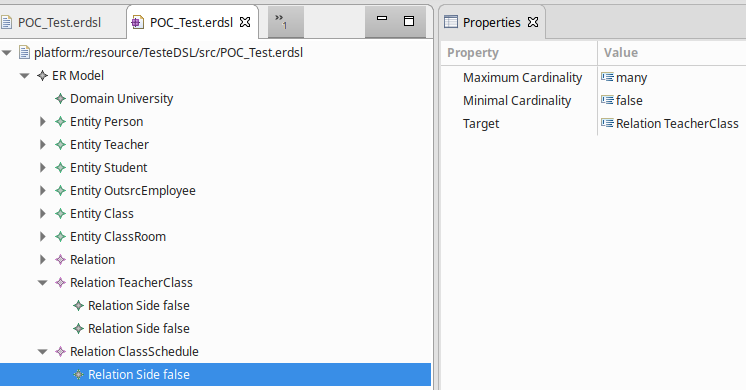
\includegraphics[width=0.9\textwidth]{img/EcoreTempoReal.png}
%     \fonte{O autor.}
% \end{figure}


%#################################################################
\section{Avaliação Preliminar da Gramática} \label{sec:AvalPrelGram}
%#################################################################
Esta seção descreve a avaliação preliminar conduzida para analisar as duas alternativas de gramática propostas, visando assim o seu aperfeiçoamento em uma versão final na solução. 

Para tanto, foi estabelecido a utilização de um grupo focal, um método de pesquisa qualitativa que objetiva gerar \textit{feedback} de um conjunto de pessoas em relação a um tema específico. 
Essa abordagem é muito utilizada como uma atividade para pesquisa de mercado em diversas áreas, uma vez que pode cumprir papel importante apoiando pesquisas exploratórias.

O processo executado nesta etapa, expressado na \autoref{fig:focusGroup}, teve como base as diretrizes estabelecidas no trabalho de \citeonline{Kontio:2008}, as quais cobrem a aplicação desse método no contexto da \ac{ES}. 

\begin{figure}[!htb]
    \centering
    \caption{Processo do Grupo Focal.}
    \label{fig:focusGroup}
    

\tikzset{every picture/.style={line width=0.75pt}} %set default line width to 0.75pt        

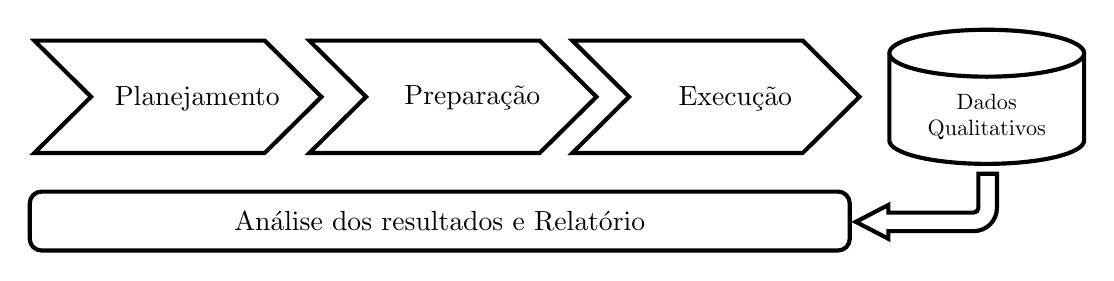
\begin{tikzpicture}[x=0.75pt,y=0.75pt,yscale=-1,xscale=1]
%uncomment if require: \path (0,300); %set diagram left start at 0, and has height of 300

%Chevron Arrow [id:dp4538178557389354] 
\draw  [line width=1.5]  (11.54,11.08) -- (122.53,11.08) -- (149.81,38.14) -- (122.53,65.19) -- (11.54,65.19) -- (38.82,38.14) -- cycle ;
%Flowchart: Magnetic Disk [id:dp3222965508094757] 
\draw  [line width=1.5]  (517.3,17.13) -- (517.3,59.14) .. controls (517.3,65.38) and (496.29,70.45) .. (470.37,70.45) .. controls (444.45,70.45) and (423.44,65.38) .. (423.44,59.14) -- (423.44,17.13)(517.3,17.13) .. controls (517.3,23.38) and (496.29,28.44) .. (470.37,28.44) .. controls (444.45,28.44) and (423.44,23.38) .. (423.44,17.13) .. controls (423.44,10.89) and (444.45,5.83) .. (470.37,5.83) .. controls (496.29,5.83) and (517.3,10.89) .. (517.3,17.13) -- cycle ;

%Chevron Arrow [id:dp4366472486660602] 
\draw  [line width=1.5]  (144.04,11.08) -- (255.03,11.08) -- (282.31,38.14) -- (255.03,65.19) -- (144.04,65.19) -- (171.32,38.14) -- cycle ;
%Chevron Arrow [id:dp3330627928283252] 
\draw  [line width=1.5]  (270.76,11.08) -- (381.75,11.08) -- (409.03,38.14) -- (381.75,65.19) -- (270.76,65.19) -- (298.04,38.14) -- cycle ;
%Rounded Rect [id:dp6923492778103744] 
\draw  [line width=1.5]  (9.3,89.48) .. controls (9.3,86.34) and (11.84,83.8) .. (14.98,83.8) -- (398.69,83.8) .. controls (401.83,83.8) and (404.37,86.34) .. (404.37,89.48) -- (404.37,106.52) .. controls (404.37,109.66) and (401.83,112.2) .. (398.69,112.2) -- (14.98,112.2) .. controls (11.84,112.2) and (9.3,109.66) .. (9.3,106.52) -- cycle ;

%Bend Arrow [id:dp33691381777556684] 
\draw  [line width=1.5]  (475.3,75.2) -- (475.3,91.64) .. controls (475.3,97.84) and (470.28,102.86) .. (464.08,102.86) -- (422.96,102.86) -- (422.96,106.52) -- (407.3,98.39) -- (422.96,90.26) -- (422.96,93.92) -- (464.08,93.92) .. controls (465.34,93.92) and (466.36,92.9) .. (466.36,91.64) -- (466.36,75.2) -- cycle ;

% Text Node
\draw (470.37,40.48) node [scale=0.8] [align=left] {Dados};
% Text Node
\draw (470.37,53.97) node [scale=0.8] [align=left] {Qualitativos};
% Text Node
\draw (90.04,38.77) node [scale=1] [align=left] {Planejamento};
% Text Node
\draw (222.54,38.77) node [scale=1] [align=left] {Preparação};
% Text Node
\draw (349.26,38.77) node [scale=1] [align=left] {Execução};
% Text Node
\draw (206.84,98) node  [align=left] {Análise dos resultados e Relatório};


\end{tikzpicture}

    \fonte{O autor.}
\end{figure}

\subsection{Planejamento}

Durante o planejamento foi definido um protocolo que deveria ser seguido.
Neste protocolo, motivado pelo problema que era gerar uma versão definitiva da gramática da \ac{DSL} proposta, foram criados os documentos necessários para sua execução: \textbf{(i)} \ac{TCLE}; \textbf{(ii)} Glossário de Termos; \textbf{(iii)} Questionário de Perfil; \textbf{(iv)} Instrumentos da Discussão 1, 2 e 3; \textbf{(v)} Modelos das Gramáticas Avaliadas; \textbf{(vi)} Roteiro de Apresentação. 
Todos os modelos dos documentos produzidos estão incluídos no \autoref{ap:GRUPOFOCAL}.

\subsubsection{Preparação}

Tipicamente as avaliações que utilizam grupos focais devem ser constituídas de quatro (4) a seis (6) grupos focais individuais para que o rigor científico seja considerado verdadeiramente alto. 
O tamanho de cada grupo focal pode variar de três (3) a até doze (12) elementos, sendo mais comum esse número ficar entre quatro (4) e oito (8) participantes \cite{Kontio:2008}. 

Por questões de viabilidade de tempo e recursos humanos, para o presente estudo foi possível ser executado um (1) grupo focal. 
Após a realização do convite houve a colaboração de treze (13) participantes, todos da área da \ac{ES}. 
Desse total, três (3) participantes eram alunos de graduação, nove (9) eram mestrandos e um (1) doutorando. 

Foi então aplicado o Questionário de Perfil, em que foi possível identificar que havia um nível equilibrado de conhecimento entre os participantes. 
Isso foi constatado pois todos já possuíam contato com \acp{DSL}, tendo utilizado esse tipo de linguagem, ao menos, durante a graduação.
Ainda foi informado que todo o processo seria gravado em áudio, fato com o qual todos concordaram.

\subsection{Execução}

O grupo focal foi realizado em 08/2019, nas dependências da UNIPAMPA, e teve duração de duas (2) horas. 
Iniciando com a exposição do roteiro que deveria ser seguido, onde houve a apresentação do objetivo do grupo focal e os conceitos básicos envolvidos, aconteceu o pedido para que os participantes realizassem a leitura e assinatura do \ac{TCLE}. 
Com o documento preenchido, foi dado continuidade ao roteiro previsto, 

A cada Instrumento de Discussão disponibilizado esperou-se até que os participantes respondessem de forma individual. 
Após, aconteceu uma discussão em grupo sobre o tema levantado. 
Todo o processo foi gravado em áudio e teve o suporte dos três (3) pesquisadores envolvidos neste estudo. 
Foi realizada também a transcrição das observações levantadas pelo debate que se seguiu, caracterizando assim as práticas de \textit{brainstorming}\footnote{\textit{Brainstorming} é uma técnica utilizada para propor soluções a um problema específico. Consiste em uma reunião, também chamada de tempestade de ideias, na qual os participantes devem ter liberdade de expor suas sugestões e debater sobre as contribuições dos colegas.} previstas em grupos focais. 

\subsection{Análise dos Resultados}

Segundo \citeonline{Kontio:2008}, a fase de análise e interpretação dos dados gerados constitui parte importante da pesquisa qualitativa, considerando o contexto, o comportamento e a percepção dos sujeitos. 
Para a fase de análise dos dados, o áudio foi analisado paralelamente as anotações realizadas.
De posse destes materiais e das respostas dos participantes para cada instrumento de discussão, foi possível avaliar os resultados do grupo focal executado.

\subsubsection{Discussões}

Após a apresentação do roteiro preparado para o grupo focal, deu-se início as discussões dos três (3) instrumentos criados para a dinâmica.
O primeiro instrumento continha a seguinte afirmação associada a uma escala Likert composta de níveis de concordância dispostos de um (1) a cinco (5):

\textit{\textbf{``Linguagens específicas de domínio com abordagem textual podem ser aplicadas na modelagem conceitual posto que conseguem descrever de forma rápida e concisa determinadas propriedades.
Sendo assim, essas soluções podem ser utilizadas ou mesmo adaptadas de uma forma efetiva no que diz respeito a representação do domínio que modelam.}}''

Após todos os participantes responderem o instrumento, foi aberto um momento de discussão entre todos. 
Por não terem visto o modelo proposto de \ac{DSL}, algumas dúvidas surgiram e os pesquisadores envolvidos procuraram sanar todas de forma a não influenciar as discussões seguintes.

O debate prosseguiu com os participantes levantando possíveis vantagens de um modelo textual.
Alguns citaram acreditar que essa abordagem poderia ser de mais fácil entendimento, porém que isso dependeria do usuário.
Esta suposição incluiu dois prováveis tipos de perfis: analistas e desenvolvedores.

O grupo chegou a conclusão que a abordagem poderia ser vista como mais produtiva por usuários de perfil desenvolvedor, mas menos proveitosa por aqueles que tivessem um viés mais analista em razão do seu nível de abstração em relação às abordagens gráficas.
A \autoref{fig:disc1GPfocalGrafico} exibe a distribuição das respostas dos participantes para a primeira discussão.

\begin{figure}[!htb]
    \centering
    \caption{Resultados da Discussão 1 - Grupo Focal.}
    \label{fig:disc1GPfocalGrafico}
    % 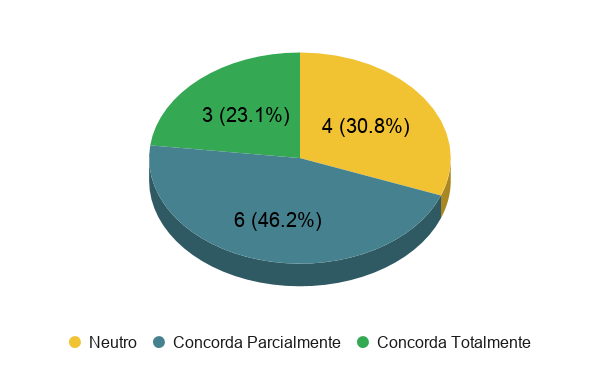
\includegraphics[width=0.8\textwidth]{img/QP1GrupoFocalGrafico.png}
    \begin{tikzpicture}
\centering
\pie 
[
    radius = 2,
    color={green!20, blue!20, orange!20}
]
    {23/\textbf{Concorda Totalmente (3)},
    30.8/\textbf{Neutro (4)}, 
    46.2/\textbf{Concorda Parcialmente (6)}}
\end{tikzpicture}

% \begin{tikzpicture}
% [
%     pie chart,
%     slice type={s1}{green}{vertical lines},
%     slice type={s2}{red}{grid},
%     slice type={s3}{orange}{sixpointed stars},
%     % slice type={s4}{purple}{bricks},
%     % slice type={s5}{blue}{vertical lines},
%     % slice type={s6}{magenta}{crosshatch dots},
%     % slice type={s7}{cyan}{horizontal lines},
%     % slice type={s8}{red}{crosshatch},
%     % slice type={s9}{brown}{dots},
%     % slice type={s10}{black}{horizontal lines},
%     pie values/.style={font={\normalsize}},
%     scale=3
% ]
%     \pie{}{23/s1,30.8/s2,46.2/s3}
%     \legend[shift={(1.2cm,1.1cm)}]{
%     {Concorda Totalmente (3)}/s1, 
%     {Neutro (4 respostas)}/s2, 
%     {Concorda Parcialmente (6)}/s3}
% \end{tikzpicture}
    \fonte{O autor.}
\end{figure}

Após, passou-se para a execução da discussão do segundo instrumento.
O atividade era composta da seguinte pergunta:

\textit{\textbf{``Considerando que um modelo conceitual de banco de dados deve definir ao menos as entidades de domínio, seus atributos e o número de ocorrências (cardinalidade) possíveis de associações (relacionamento), como você definiria uma gramática básica (DSL) para a sua representação?''}}

Foi informado que os participantes poderiam conversar livremente durante toda a realização deste exercício.
Após cada um sugerir a sua sintaxe, houve debate e troca de informações sobre como estruturar melhor as informações. 
A discussão foi focada principalmente em como representar as relações do modelo \ac{ER} em uma sintaxe textual. 

A maior dificuldade se mostrou em como definir uma ordem. 
Outro ponto que merece destaque foi quanto à cardinalidade, onde no geral seguiu-se a nomenclatura utilizada no diagrama original de Chen (\textit{e.g.} 0,1). 
Entretanto, ao fim do instrumento houveram opiniões muito divergentes em relação à representação ideal. 
Aparentemente, cada um teve uma visão distinta, alguns optando por incluir as relações dentro das entidades, e outros fora. 

Aconteceram também sugestões quanto às palavras-chave possíveis, como \texttt{Element}, \texttt{ElementFather}, \texttt{ElementSource}, \texttt{Type}, e \texttt{Referential}.
Ainda, seis (6) participantes sugeriram o uso de ponto e vírgula (;) para separação das declarações de elementos, e todos os treze (13) preconizaram a utilização de símbolos como parênteses, colchetes e/ou chaves para agrupar conjuntos similares de elementos.				

Finalizada a dinâmica proposta, chegou-se ao último instrumento do grupo focal.
Este artefato era composto de um exemplo de cada versão da gramática (Apêndice \ref{ap:ModelosGP}) produzida preliminarmente para este trabalho.
De posse das versões, foi pedido que os participantes realizassem a escolha entre as opções, apontando assim qual avaliavam como mais viável para modelagem \ac{ER}.
Também foi solicitado que fossem indicados os pontos positivos e negativos observados em cada modelo.

O segundo modelo acabou por ser escolhido pela maioria, como pode ser observado na \autoref{fig:disc3GPfocalGrafico}.
Porém, ao final das discussões obteve-se um consenso de que a forma de definição de entidades do primeiro modelo e a disposição dos relacionamentos do segundo, em especial o uso das convenções nas cardinalidades, eram os mais adequado para a aplicação no ensino, indicando assim a necessidade de uma fusão de ambas as versões.

\begin{figure}[!htb]
    \centering
    \caption{Resultados da Discussão 3 - Grupo Focal.}
    \label{fig:disc3GPfocalGrafico}
    % 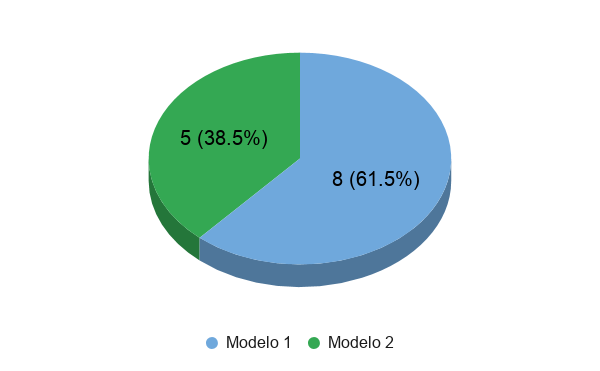
\includegraphics[width=0.8\textwidth]{img/QP3GrupoFocalGrafico.png}
    \begin{tikzpicture}
\centering
\pie
[
    radius = 2,
    color={green!20, orange!20}
]
    {38.5/\textbf{Modelo 1 (5)},
    61.5/\textbf{Modelo 2 (8)}}
\end{tikzpicture}
    \fonte{O autor.}
\end{figure}

%Levantou-se como uma possível vantagem a possibilidade de os clientes poderem representar um modelo ER textualmente, estando em aderência com as práticas do DevOps que necessita dessa interação frequente com stakeholders não técnicos. Levantou-se novamente a necessidade de integrar a representação textual com a de Chen e as cores dos diferentes comandos.

%#################################################################
\section{A Ferramenta ERText} \label{sec:ERTEXTFinal}
%#################################################################

Esta seção apresenta a ferramenta com o \textit{plugin} final da solução proposta. 
Este \textit{plugin} pode tanto ser integrado com a \ac{RCP} Eclipse, como pode ser insumo para um aplicativo independente (\textit{standalone application}).

A diferença é que quando usado como um \textit{plugin} do Eclipse o editor pode fornecer, além das funcionalidades da gramática, suporte a outras linguagens \textit{e.g.} Java, PHP. 
Um produto independente, por outro lado, fornece toda a infraestrutura voltada unicamente a linguagem desenvolvida, e pode ser distribuído como uma ferramenta livre desde que seguidas as diretrizes da licença de software EPL-2.0\footnote{https://www.eclipse.org/legal/epl-2.0/}.

\subsection{Operação da ERText}

Como dito anteriormente, a versão final da gramática resultou da fusão entre os duas versões previamente definidas e avaliadas com a execução do grupo focal.
As principais mudanças foram as modificações das palavras reservadas \texttt{isA} e \texttt{isRelatedWith} por \texttt{is} e \texttt{relates}, respectivamente, além da adoção da convenção \texttt{(0:1) (1:1) (0:N) (1:N)} para as cardinalidades.

% \begin{figure}
%     \centering
%     \caption{Versão final da \ac{DSL}.}
%     \label{fig:DSLFINAL}
%     \begin{scriptsize}
%     \begin{lstlisting}[language = Xtext , frame = trbl]
% grammar org.xtext.unipampa.erdsl.ErDsl with org.eclipse.xtext.common.Terminals

% generate erDsl "http://www.xtext.org/unipampa/erdsl/ErDsl"

% ERModel:
% 	domain=Domain ';'
% 	('Entities' '{') entities+=Entity+ ('}' ';')
% 	('Relationships' '{') relations+=Relation* ('}' ';');
	
% Domain:
% 	'Domain' name=ID;

% Attribute:
%         name=ID type=DataType (isKey?='isIdentifier')?;

% enum DataType:
%         INT='int' | DOUBLE='double' |
%         MONEY='money' | STRING='string' | 
%         BOOLEAN='boolean' | DATETIME='datetime' | BLOB='file';

% Entity:
% 	name=ID ('is' is+=[Entity])*
% 	('{' attributes+=Attribute (',' attributes+=Attribute)* '}')?;

% Relation:
% 	(name=ID)? ('[' leftEnding=RelationSide 
% 	'relates' rightEnding=RelationSide ']') 
% 	('{'attributes+=Attribute (',' attributes+=Attribute)* '}')*;


% RelationSide:
% 	Cardinality=('(0:1)' | '(1:1)' | '(0:N)' | '(1:N)') 
% 	target=[Entity] | target=[Relation];
    
%     \end{lstlisting}
%     \end{scriptsize}    
%     \fonte{O autor.}
% \end{figure}

Após o \textit{plugin} ser integrado no \ac{RCP}, é possível verificar sua instalação no ambiente conforme exposto na \autoref{fig:pluginInstalado}.

\begin{figure}[!htb]
    \centering
    \caption{Fragmento do \textit{plugin} da solução instalado.}
    \label{fig:pluginInstalado}
    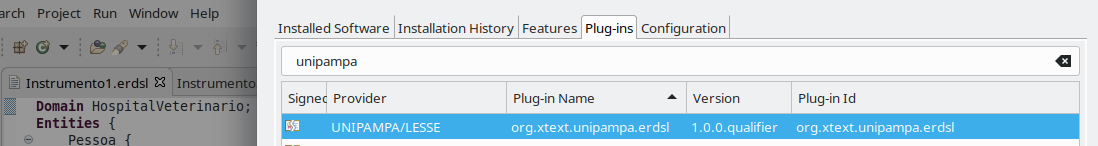
\includegraphics[width=\textwidth]{img/PluginInstalado}
    \fonte{O autor.}
\end{figure}

A \autoref{fig:ERTextUso} apresenta a ferramenta em funcionamento, onde é possível ser feita a criação de arquivos de modelagem utilizando a \ac{DSL}. 
Neste exemplo há a modelagem de sete (7) entidades e seis (6) relacionamentos, incluindo um autorelacionamento e um relacionamento ternário.

A modelagem na ferramenta ganha validação em tempo real,  \textit{syntax highlighting}, que indica erros de sintaxe em tempo de escrita, autocomplemento de código e \textit{hovering}, uma funcionalidade que exibe informações sobre um item quando o cursor do \textit{mouse} é colocado sobre ele.

Se sabe que a definição dos tipos de dados não é prevista no modelo conceitual clássico mas, por questões relacionados a pretensão futura de realizar a geração de instruções \ac{SQL}, foi decido pela manutenção dessa escolha de projeto. 

\begin{figure}[!htb]
    \centering
    \caption{Fragmento da solução sendo utilizada.}
    \label{fig:ERTextUso}
    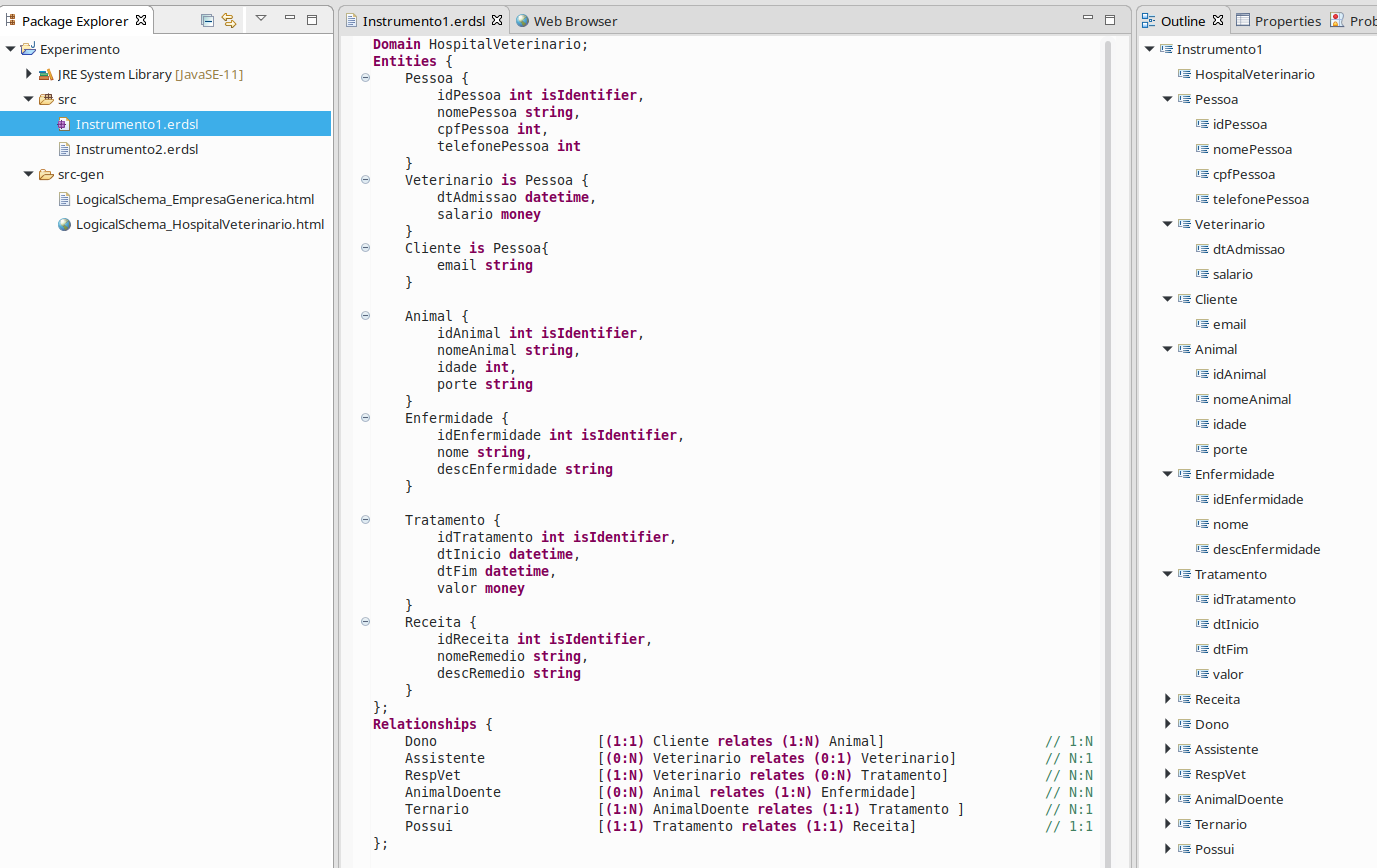
\includegraphics[width=0.95\textwidth]{img/ERTextUso}
    \fonte{O autor.}
\end{figure}

A função para o mapeamento e geração do modelo lógico é executada automaticamente toda a vez que uma modelo é salvo.
Na figura anterior pode-se observar os arquivos \textit{.html} na estrutura de diretórios na guia da esquerda, dentro da pasta \textit{src-gen}.
Foram gerados arquivos com esse formato para uma melhor visualização a partir de marcações no texto.

Estas marcações podem ser renderizadas por qualquer navegador de Internet, ou mesmo dentro do próprio ambiente, aumentando o poder de compreensão por parte do usuário.
O modelo lógico derivado pelo gerador que mapeia o modelo conceitual é apresentado na \autoref{fig:modeloLogico}.

\begin{figure}[!htb]
    \centering
    \caption{Exemplo de modelo lógico gerado.}
    \label{fig:modeloLogico}
    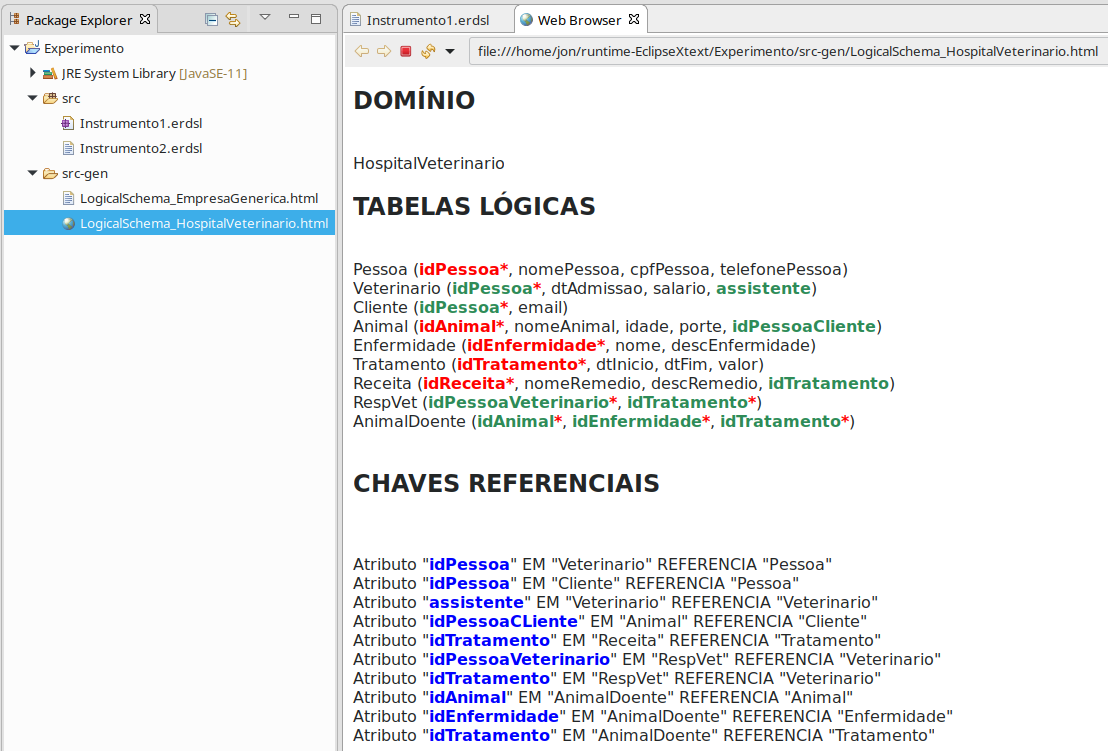
\includegraphics[width=0.95\textwidth]{img/ModeloLogico}
    \fonte{O autor.}
\end{figure}

Mediante as premissas assumidas para a realização da transformação, o modelo original resulta em um novo modelo composto de nove (9) entidades, e também já possuindo suas integridade referenciais inferidas, ou seja, os registros que apontam para outros registros já são estabelecidos. 

É importante salientar que as premissas foram escolhidas previamente com base no livro referência de \citeonline{Heuser:2009}.
A \autoref{fig:Premissas} expõe as alternativas de mapeamento entre os modelos, sendo que as assinaladas são as que foram implementadas até o momento da entrega deste estudo.
Em relação ao conceito de generalização/especialização, também foi necessário assumir uma ideia inicial que teria que ser tomada como verdade.

% \begin{figure}[!htb]
%     \centering
%     \caption{Fragmento do gerador desenvolvido para o mapeamento lógico.}
%     \label{fig:GeradorXtend}
%     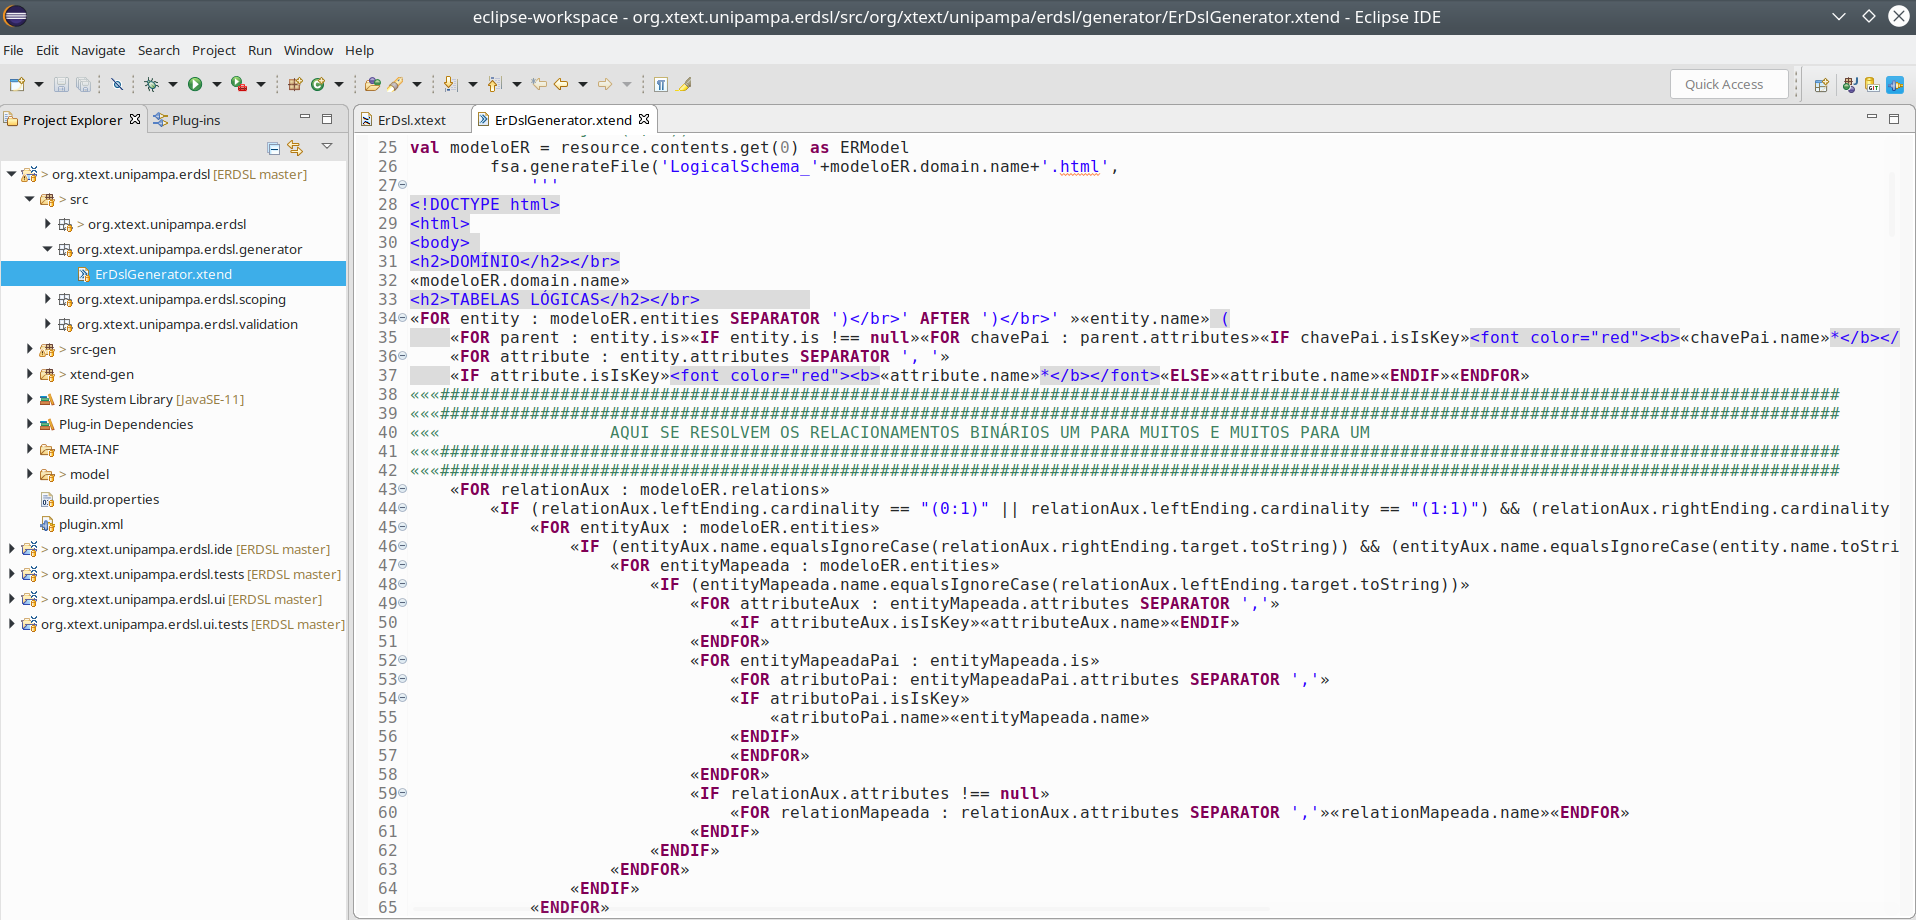
\includegraphics[width=\textwidth]{img/GeradorXtend}
%     \fonte{O autor.}
% \end{figure}

\begin{figure}[!htb]
    \centering
    \caption{Premissas adotadas para a transformação entre os modelos.}
    \label{fig:Premissas}
    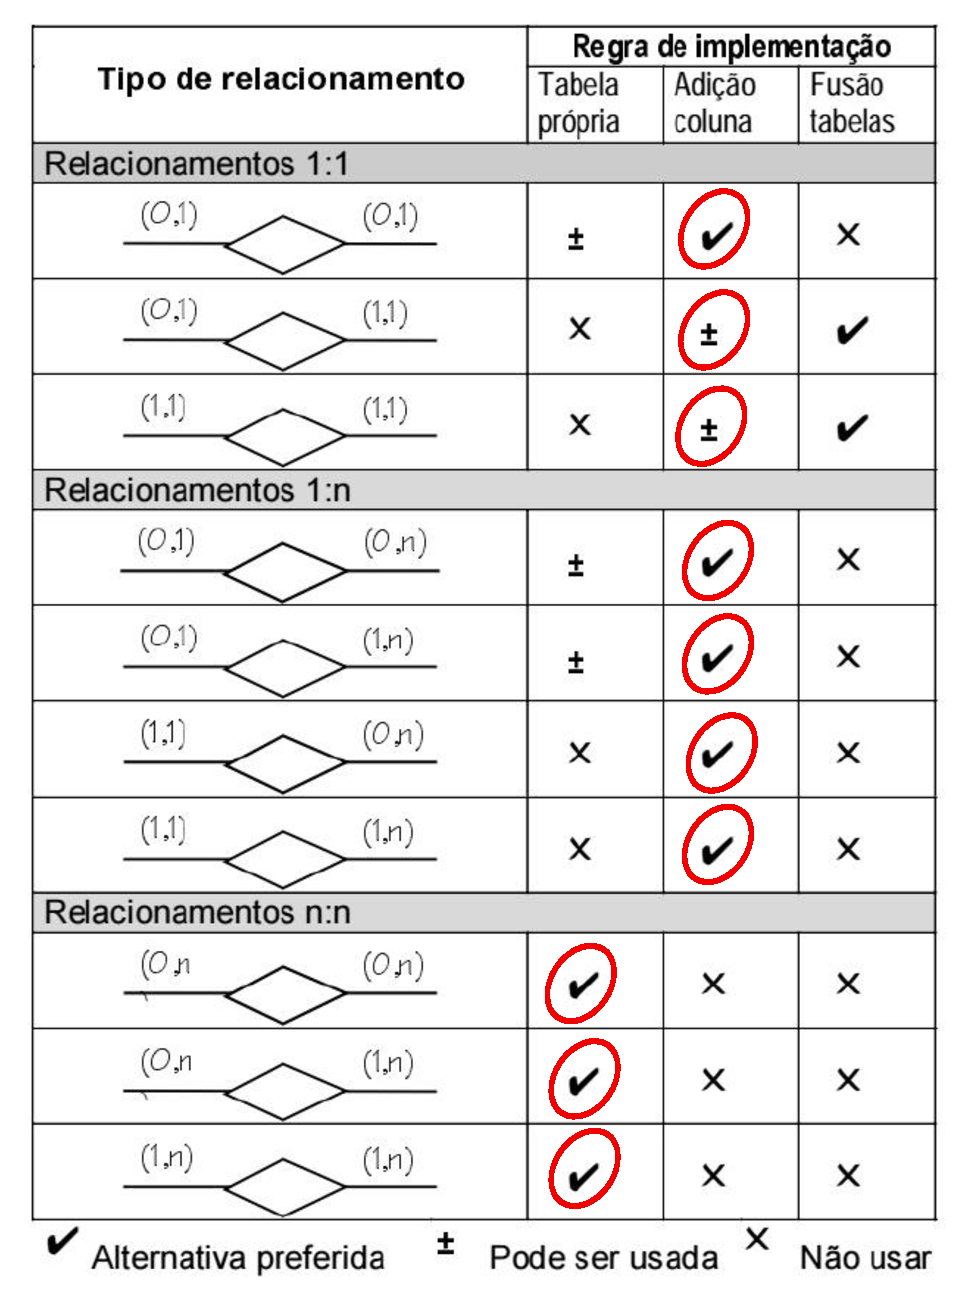
\includegraphics[width=0.5\textwidth]{img/EPS/TabelaMapeamentoRelacionamentos}
    \fonte{\citeonline{Heuser:2009}.}
\end{figure}

Segundo \citeonline{Heuser:2009}, para estes casos existe duas alternativas passíveis de serem derivadas. 
A primeira recomenda o uso de uma única tabela para toda a hierarquia de entidades, ou seja, recomenda a fusão das tabelas.
A segunda recomenda o uso de uma tabela por entidade modelada, desde que respeitado a integridade referencial, ou seja, as chaves primárias das entidades filhas devem apontar necessariamente para a chave primária da entidade pai. 
No caso da ferramenta resultante neste trabalho, optou-se pela segunda alternativa. 

O gerador do modelo lógico foi desenvolvido com a \ac{GPL} Xtend, e atualmente conta com cerca de quatrocentas linhas de código para realizar a transformação do modelo conceitual para o modelo lógico. 





%#################################################################
\section{Lições do Capítulo} \label{sec:licDSL}
%#################################################################

Neste capítulo foram expostos os requisitos, as decisões de projeto e a arquitetura da \ac{DSL} proposta para a solução desenvolvida. 
Também foi demonstrado como o protótipo da versão preliminar da linguagem foi definido, um exemplo de uso e o grupo focal conduzido para a avaliação preliminar.

Com base nos resultados do grupo focal, foi possível chegar na versão final da \ac{DSL} proposta, realizando então a sua implementação como um \textit{plugin} integrado em um \ac{RCP} Eclipse, gerando assim a ferramenta ERText.
Desta forma o processo de modelagem com a nova linguagem criada ganhou recursos nativos como autocomplemento de código, formatação, validação com base nas restrições descritas na gramática e \textit{syntax highlighting}.

Por fim, o projeto desta solução está disponível publicamente, sob a licença EPL-2.0, no \textit{ProjetoDSL}\footnote{Repositório ERDSL: \url{https://github.com/ProjetoDSL/ERDSL}}, pertencente ao grupo de pesquisa \textit{Laboratory of Empirical Studies in Software Engineering} (LESSE) da UNIPAMPA.

% Até o momento o Xtext mostrou-se uma \ac{LW} capaz de suprir as necessidades iniciais do projeto, fornecendo suporte completo para a criação de gramáticas com notação \ac{BNF}, uma meta-sintaxe amplamente usada para expressar gramáticas livres de contexto como nas estruturas de linguagens de programação no geral. 
% Além de prover a validação da gramática criada, foi gerado um \textit{plugin} tornando assim possível a realização do teste do protótipo em um \ac{RCP} Eclipse. 

% Assim, por meio disso o processo de modelagem com a nova linguagem criada ganhou recursos nativos como formatação, validação com base nas restrições descritas na gramática e \textit{syntax highlighting}. 
%É importante ressaltar que o \textit{plugin} somente pôde ser testado devido a integração nativa fornecida pelo Xtext com o \ac{EMF}, um conjunto de recursos do Eclipse para representar modelos e gerar código equivalente. 